\section*{Software Information}

\begin{itemize}
\item Please check, whether your inputs, the equations applied and the charactersitics are displayed correctly.
\item You are welcome to send your feedback via \url{https://github.com/oemof/tespy/issues}.
\item \LaTeX packages required are:
\begin{itemize}
\item graphicx
\item float
\item hyperref
\item booktabs
\item amsmath
\item units
\item cleveref
\end{itemize}
\item To supress these messages, call the model documentation with the keyword draft=False.
\end{itemize}

\begin{table}[H]
\begin{tabular}{ll}
TESPy Version:&0.4.3 - dev\\
Commit:&b8e11e11@dev\\
CoolProp version:&6.4.0\\
Python version:&3.7.6 (default, Jan  8 2020, 20:23:39) [MSC v.1916 64 bit (AMD64)]\\
Documentation generated:&Februar 22, 2021\\
\end{tabular}
\end{table}
\newpage\section{Connections in offdesign mode}

\subsection{Specified connection parameters}

\begin{table}[H]\begin{center}
\begin{tabular}{lrrr}
\toprule
                                                          label &  p in $\unit[]{bar}$ (\ref{eq:Connection_pressure}) &  T in $\unit[]{^\circ C}$ (\ref{eq:Connection_temperature}) &  m in $\unitfrac[]{kg}{s}$ (\ref{eq:Connection_mass flow}) \\
\midrule
                               ambient air:out1\_compressor:in1 &                                               1.000 &                                                      20.000 &                                                          - \\
                                   economizer:out1\_chimney:in1 &                                               1.020 &                                                           - &                                                          - \\
                     cooling water backflow:out1\_condenser:in2 &                                               5.000 &                                                      15.000 &                                                          - \\
                     condenser:out2\_cooling water feedflow:in1 &                                                   - &                                                           - &                                                   1213.429 \\
 district heating backflow:out1\_district heating condenser:in2 &                                              10.000 &                                                      50.000 &                                                          - \\
 district heating condenser:out2\_district heating feedflow:in1 &                                                   - &                                                      90.000 &                                                          - \\
\bottomrule
\end{tabular}
\caption{Specified connection parameters}
\end{center}\end{table}

\subsection{Equations applied}

\begin{equation}
\label{eq:Connection_pressure}
0 = p - p_\mathrm{spec}
\end{equation}

\begin{equation}
\label{eq:Connection_temperature}
0 = T \left(p, h \right) - T_\mathrm{spec}
\end{equation}

\begin{equation}
\label{eq:Connection_mass flow}
0 = \dot{m} - \dot{m}_\mathrm{spec}
\end{equation}

\subsection{Specified fluids}

\begin{table}[H]\begin{center}
\begin{tabular}{lrrrrrr}
\toprule
                                                          label &  Ar (\ref{eq:Connection_Ar}) &  CH4 (\ref{eq:Connection_CH4}) &  CO2 (\ref{eq:Connection_CO2}) &  H2O (\ref{eq:Connection_H2O}) &  N2 (\ref{eq:Connection_N2}) &  O2 (\ref{eq:Connection_O2}) \\
\midrule
                               ambient air:out1\_compressor:in1 &                        0.013 &                          0.000 &                          0.000 &                          0.000 &                        0.755 &                        0.231 \\
                          fuel source:out1\_fuel compressor:in1 &                        0.000 &                          0.960 &                          0.040 &                          0.000 &                        0.000 &                        0.000 \\
                                  superheater:out2\_ls sink:in1 &                        0.000 &                          0.000 &                          0.000 &                          1.000 &                        0.000 &                        0.000 \\
                     cooling water backflow:out1\_condenser:in2 &                        0.000 &                          0.000 &                          0.000 &                          1.000 &                        0.000 &                        0.000 \\
 district heating backflow:out1\_district heating condenser:in2 &                        0.000 &                          0.000 &                          0.000 &                          1.000 &                        0.000 &                        0.000 \\
\bottomrule
\end{tabular}
\caption{Specified fluids}
\end{center}\end{table}

\subsection{Equations applied}

\begin{equation}
\label{eq:Connection_Ar}
0 = x_\mathrm{Ar} - x_\mathrm{Ar,spec}
\end{equation}

\begin{equation}
\label{eq:Connection_CH4}
0 = x_\mathrm{CH4} - x_\mathrm{CH4,spec}
\end{equation}

\begin{equation}
\label{eq:Connection_CO2}
0 = x_\mathrm{CO2} - x_\mathrm{CO2,spec}
\end{equation}

\begin{equation}
\label{eq:Connection_H2O}
0 = x_\mathrm{H2O} - x_\mathrm{H2O,spec}
\end{equation}

\begin{equation}
\label{eq:Connection_N2}
0 = x_\mathrm{N2} - x_\mathrm{N2,spec}
\end{equation}

\begin{equation}
\label{eq:Connection_O2}
0 = x_\mathrm{O2} - x_\mathrm{O2,spec}
\end{equation}

\subsection{Referenced values for mass flow}

\begin{table}[H]\begin{center}
\begin{tabular}{llrr}
\toprule
                     label &                   reference &  factor in - &  delta in $\unitfrac[]{kg}{s}$ \\
\midrule
 evaporator:out2\_drum:in2 &  drum:out2\_superheater:in2 &            4 &                              0 \\
\bottomrule
\end{tabular}
\caption{Referenced values for mass flow}
\end{center}\end{table}

\subsection{Equation applied}

\begin{equation}
\label{eq:Connection_ref}
0 = \text{value} - \text{value}_\mathrm{ref} \cdot \mathrm{factor} + \text{delta}
\end{equation}

\subsection{Referenced values for pressure}

\begin{table}[H]\begin{center}
\begin{tabular}{llrr}
\toprule
                                           label &                         reference &  factor in - &  delta in $\unit[]{bar}$ \\
\midrule
           fuel source:out1\_fuel compressor:in1 &  ambient air:out1\_compressor:in1 &            1 &                        0 \\
 ls source:out1\_steam turbine high pressure:in1 &     superheater:out2\_ls sink:in1 &            1 &                        0 \\
\bottomrule
\end{tabular}
\caption{Referenced values for pressure}
\end{center}\end{table}

\subsection{Equation applied}

\begin{equation}
\label{eq:Connection_ref}
0 = \text{value} - \text{value}_\mathrm{ref} \cdot \mathrm{factor} + \text{delta}
\end{equation}

\subsection{Referenced values for enthalpy}

\begin{table}[H]\begin{center}
\begin{tabular}{llrr}
\toprule
                                           label &                      reference &  factor in - &  delta in $\unitfrac[]{kJ}{kg}$ \\
\midrule
 ls source:out1\_steam turbine high pressure:in1 &  superheater:out2\_ls sink:in1 &            1 &                               0 \\
\bottomrule
\end{tabular}
\caption{Referenced values for enthalpy}
\end{center}\end{table}

\subsection{Equation applied}

\begin{equation}
\label{eq:Connection_ref}
0 = \text{value} - \text{value}_\mathrm{ref} \cdot \mathrm{factor} + \text{delta}
\end{equation}

\subsection{Referenced values for temperature}

\begin{table}[H]\begin{center}
\begin{tabular}{llrr}
\toprule
                                 label &                         reference &  factor in - &  delta in $\unit[]{^\circ C}$ \\
\midrule
 fuel source:out1\_fuel compressor:in1 &  ambient air:out1\_compressor:in1 &            1 &                             0 \\
\bottomrule
\end{tabular}
\caption{Referenced values for temperature}
\end{center}\end{table}

\subsection{Equation applied}

\begin{equation}
\label{eq:Connection_ref}
0 = \text{value} - \text{value}_\mathrm{ref} \cdot \mathrm{factor} + \text{delta}
\end{equation}

\section{User defined equations in offdesign mode}

\section{Components in offdesign mode}

\subsection{Components of type Compressor}

\subsubsection{Mandatory constraints}

\begin{equation}
\label{eq:Compressor_mass_flow_constraints}
0=\dot{m}_{\mathrm{in,}i}-\dot{m}_{\mathrm{out,}i}\; \forall i \in [1]
\end{equation}

\begin{equation}
\label{eq:Compressor_fluid_constraints}
0=x_{fl\mathrm{,in,}i}-x_{fl\mathrm{,out,}i}\;\forall fl \in\text{network fluids,}\; \forall i \in [1]
\end{equation}


\subsubsection{Inputs specified}

\begin{table}[H]\begin{center}
\begin{tabular}{ll}
\toprule
           label &  eta\_s\_char (\ref{eq:Compressor_eta_s_char}) \\
\midrule
      compressor &                                           True \\
 fuel compressor &                                           True \\
\bottomrule
\end{tabular}
\caption{Parameters of components of type Compressor}
\end{center}\end{table}

\subsubsection{Equations applied}

\begin{equation}
\label{eq:Compressor_eta_s_char}
0=\left(h_\mathrm{out}-h_\mathrm{in}\right)\cdot\eta_\mathrm{s,design}\cdot f\left(X\right)-\left( h_{out,s} - h_{in} \right)
\end{equation}

\begin{minipage}{0.5\textwidth}
\begin{figure}[H]\begin{center}
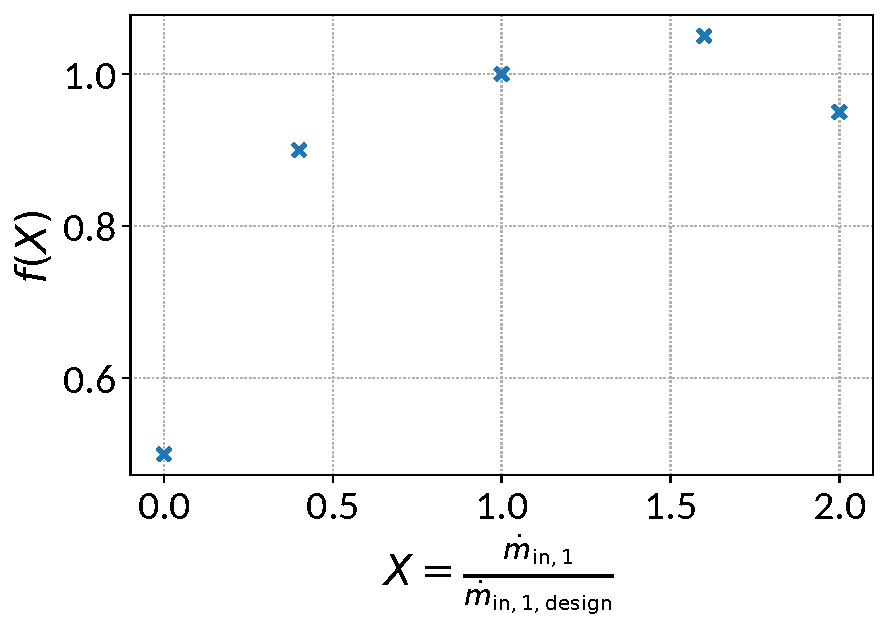
\includegraphics[width=\textwidth]{figures/Compressor_CharLine_eta_s_char_compressor.pdf}
\caption{Characteristics of compressor (eq. \ref{eq:Compressor_eta_s_char})}
\label{fig:CharLine_eta_s_char_compressor}
\end{center}\end{figure}

\end{minipage}
\begin{minipage}{0.5\textwidth}
\begin{figure}[H]\begin{center}
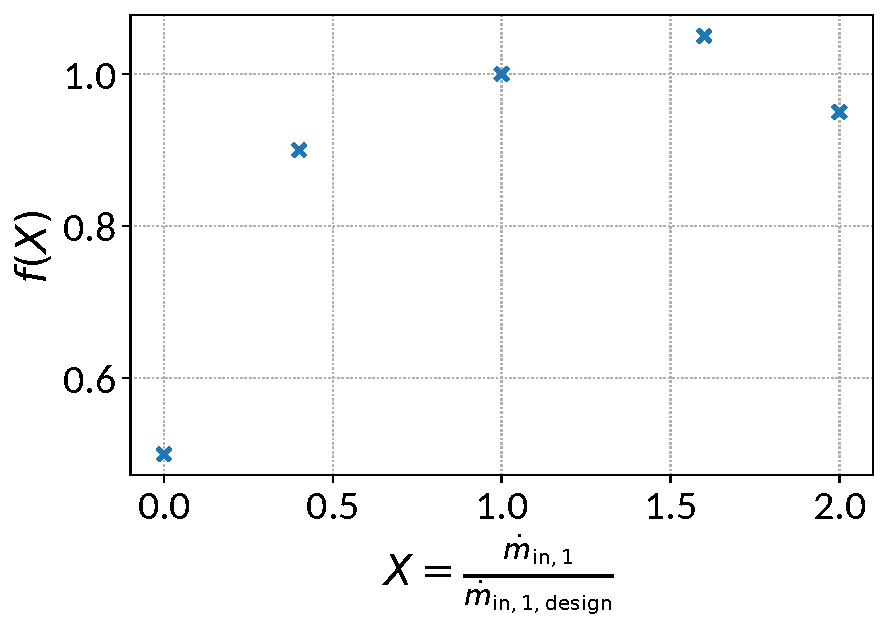
\includegraphics[width=\textwidth]{figures/Compressor_CharLine_eta_s_char_fuel_compressor.pdf}
\caption{Characteristics of fuel compressor (eq. \ref{eq:Compressor_eta_s_char})}
\label{fig:CharLine_eta_s_char_fuel compressor}
\end{center}\end{figure}

\end{minipage}


\subsection{Components of type CombustionChamber}

\subsubsection{Mandatory constraints}

\begin{equation}
\label{eq:CombustionChamber_mass_flow_constraints}
0=\dot{m}_\mathrm{in,1} + \dot{m}_\mathrm{in,2} - \dot{m}_\mathrm{out,1}
\end{equation}

\begin{equation}
\label{eq:CombustionChamber_reactor_pressure_constraints}
\begin{split}
0 = & p_\mathrm{in,1} - p_\mathrm{out,1}\\
0 = & p_\mathrm{in,1} - p_\mathrm{in,2}\\
\end{split}
\end{equation}

\begin{equation}
\label{eq:CombustionChamber_stoichiometry_constraints_general_eq}
\begin{split}
&\Delta \dot{m}_\mathrm{fluid} = \dot{m}_\mathrm{in,1} \cdot x_\mathrm{fluid,in,1} +\dot{m}_\mathrm{in,2} \cdot x_\mathrm{fluid,in,2}-\dot{m}_\mathrm{out,1} \cdot x_\mathrm{fluid,out,1}\\
&\dot{m}_\mathrm{fluid,m} = \frac{\dot{m}_\mathrm{in,1} \cdot x_\mathrm{fluid,in,1} +\dot{m}_\mathrm{in,2} \cdot x_\mathrm{fluid,in,2}}{M_\mathrm{fluid}}\\
&\dot{m}_\mathrm{H,m}=\dot{m}_\mathrm{CH4,m} \cdot 4\\
&\dot{m}_\mathrm{C,m}=\dot{m}_\mathrm{CH4,m} \cdot 1\\
&\dot{m}_\mathrm{O2,m,stoich}=\frac{\dot{m}_\mathrm{H,m}}{4} + \dot{m}_\mathrm{C,m}\\
\end{split}
\end{equation}
\begin{equation}
\label{eq:CombustionChamber_stoichiometry_constraints_Ar}
0 = \Delta \dot{m}_\mathrm{Ar}
\end{equation}
\begin{equation}
\label{eq:CombustionChamber_stoichiometry_constraints_CH4}
0=\Delta\dot{m}_\mathrm{CH4}-\dot{m}_\mathrm{CH4,m} \cdot M_\mathrm{CH4}
\end{equation}
\begin{equation}
\label{eq:CombustionChamber_stoichiometry_constraints_CO2}
0=\Delta \dot{m}_\mathrm{CO2} + \dot{m}_\mathrm{C,m} \cdot M_\mathrm{CO2} 
\end{equation}
\begin{equation}
\label{eq:CombustionChamber_stoichiometry_constraints_H2O}
0=\Delta \dot{m}_\mathrm{H2O} + \frac{\dot{m}_\mathrm{H,m}}{2} \cdot M_\mathrm{H2O} 
\end{equation}
\begin{equation}
\label{eq:CombustionChamber_stoichiometry_constraints_N2}
0 = \Delta \dot{m}_\mathrm{N2}
\end{equation}
\begin{equation}
\label{eq:CombustionChamber_stoichiometry_constraints_O2}
0=\Delta\dot{m}_\mathrm{O2}-\dot{m}_\mathrm{O2,m,stoich} \cdot M_\mathrm{O2}
\end{equation}

\begin{equation}
\label{eq:CombustionChamber_energy_balance_constraints}
\begin{split}
0 = & \sum_i \dot{m}_{\mathrm{in,}i} \cdot\left( h_{\mathrm{in,}i} - h_{\mathrm{in,}i\mathrm{,ref}} \right) -\dot{m}_\mathrm{out,1}\cdot\left( h_\mathrm{out,1} - h_\mathrm{out,1,ref}\right)\\
& + LHV_{fuel} \cdot \left(\sum_i \dot{m}_{\mathrm{in,}i} \cdot x_{fuel\mathrm{,in,}i} - \dot{m}_\mathrm{out,1} \cdot x_{fuel\mathrm{,out,1}} \right)\\
& \forall i \in \text{inlets}\\& T_\mathrm{ref}=\unit[298.15]{K}\;p_\mathrm{ref}=\unit[10^5]{Pa}\\
\end{split}
\end{equation}


\subsubsection{Inputs specified}

\begin{table}[H]\begin{center}
\begin{tabular}{lr}
\toprule
      label &  lamb (\ref{eq:CombustionChamber_lamb}) \\
\midrule
 combustion &                                   2.500 \\
\bottomrule
\end{tabular}
\caption{Parameters of components of type CombustionChamber}
\end{center}\end{table}

\subsubsection{Equations applied}

\begin{equation}
\label{eq:CombustionChamber_lamb}
\begin{split}
0 = \frac{\dot{m}_\mathrm{fuel,m}}{\dot{m}_\mathrm{O_2,m} \cdot \left(n_\mathrm{C,fuel} + 0.25 \cdot n_\mathrm{H,fuel}\right)} - \lambda \\
\dot{m}_\mathrm{fluid,m} = \frac{x_\mathrm{fluid} \cdot \dot{m}}{M_\mathrm{fluid}}\\
\end{split}
\end{equation}


\subsection{Components of type Turbine}

\subsubsection{Mandatory constraints}

\begin{equation}
\label{eq:Turbine_mass_flow_constraints}
0=\dot{m}_{\mathrm{in,}i}-\dot{m}_{\mathrm{out,}i}\; \forall i \in [1]
\end{equation}

\begin{equation}
\label{eq:Turbine_fluid_constraints}
0=x_{fl\mathrm{,in,}i}-x_{fl\mathrm{,out,}i}\;\forall fl \in\text{network fluids,}\; \forall i \in [1]
\end{equation}


\subsubsection{Inputs specified}

\begin{table}[H]\begin{center}
\begin{tabular}{lll}
\toprule
                       label &  eta\_s\_char (\ref{eq:Turbine_eta_s_char}) &  cone (\ref{eq:Turbine_cone}) \\
\midrule
                 gas turbine &                                        True &                          True \\
 steam turbine high pressure &                                        True &                          True \\
  steam turbine low pressure &                                        True &                          True \\
\bottomrule
\end{tabular}
\caption{Parameters of components of type Turbine}
\end{center}\end{table}

\subsubsection{Equations applied}

\begin{equation}
\label{eq:Turbine_eta_s_char}
0=-\left(h_\mathrm{out}-h_\mathrm{in}\right)+\eta_\mathrm{s,design}\cdot f \left(X\right)\cdot\left(h_\mathrm{out,s}-h_\mathrm{in}\right)
\end{equation}

\begin{equation}
\label{eq:Turbine_cone}
0 = \frac{\dot{m}_\mathrm{in,design}\cdot p_\mathrm{in}}{p_\mathrm{in,design}}\cdot\sqrt{\frac{p_\mathrm{in,design}\cdot v_\mathrm{in}}{p_\mathrm{in}\cdot v_\mathrm{in,design}}\cdot\frac{1-\left(\frac{p_\mathrm{out}}{p_\mathrm{in}} \right)^{2}}{1-\left(\frac{p_\mathrm{out,design}}{p_\mathrm{in,design}}\right)^{2}}} -\dot{m}_\mathrm{in}
\end{equation}

\begin{minipage}{0.5\textwidth}
\begin{figure}[H]\begin{center}
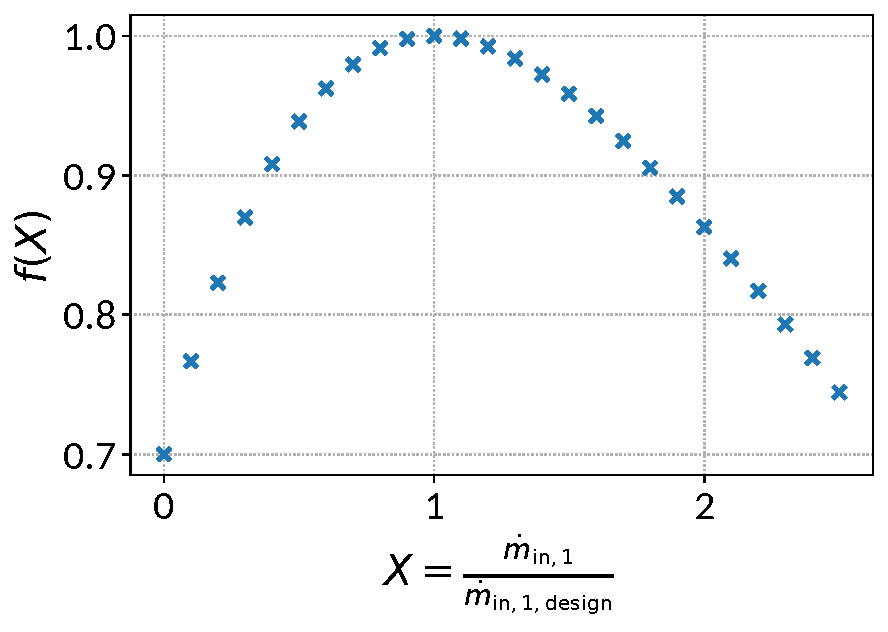
\includegraphics[width=\textwidth]{figures/Turbine_CharLine_eta_s_char_gas_turbine.pdf}
\caption{Characteristics of gas turbine (eq. \ref{eq:Turbine_eta_s_char})}
\label{fig:CharLine_eta_s_char_gas turbine}
\end{center}\end{figure}

\end{minipage}
\begin{minipage}{0.5\textwidth}
\begin{figure}[H]\begin{center}
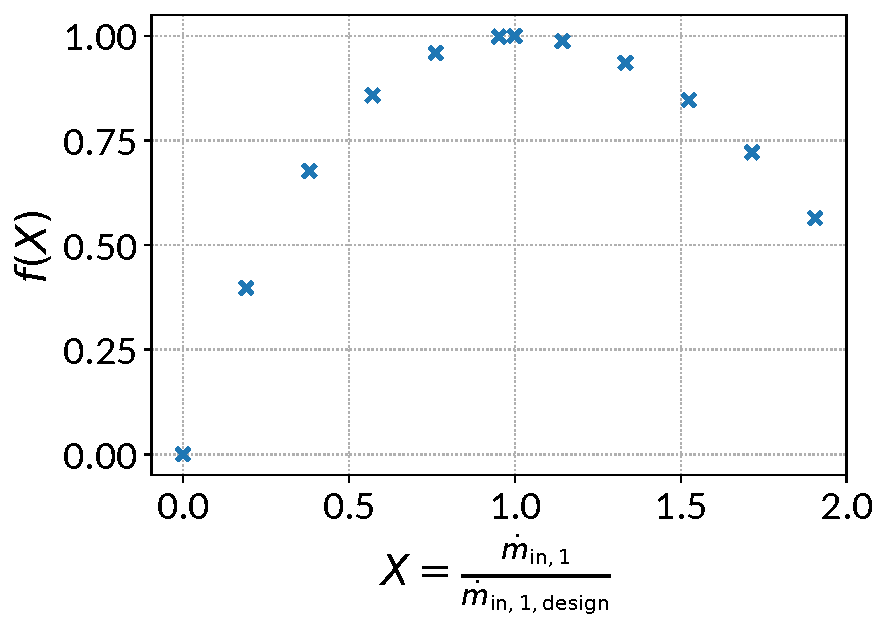
\includegraphics[width=\textwidth]{figures/Turbine_CharLine_eta_s_char_steam_turbine_high_pressure.pdf}
\caption{Characteristics of steam turbine high pressure (eq. \ref{eq:Turbine_eta_s_char})}
\label{fig:CharLine_eta_s_char_steam turbine high pressure}
\end{center}\end{figure}

\end{minipage}

\begin{minipage}{0.5\textwidth}
\begin{figure}[H]\begin{center}
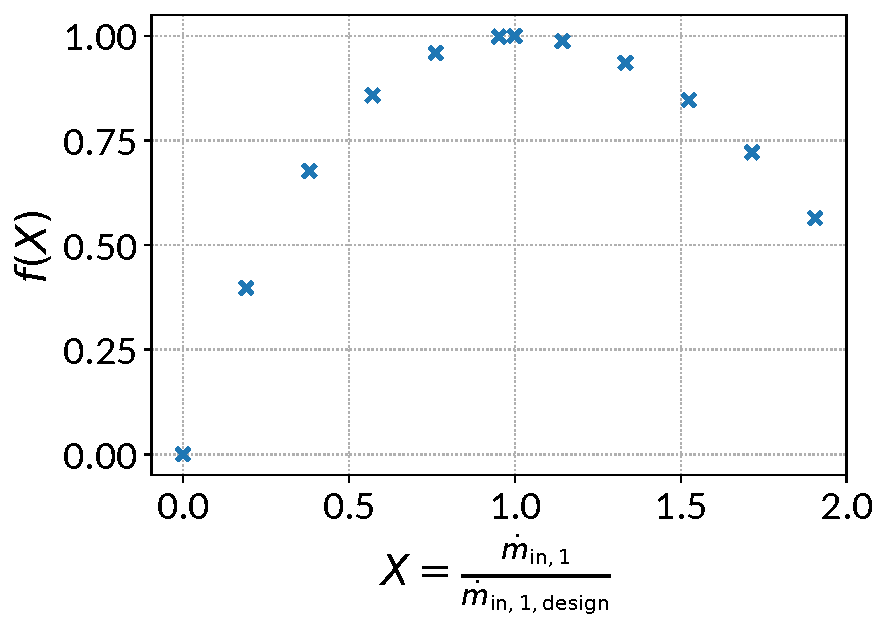
\includegraphics[width=\textwidth]{figures/Turbine_CharLine_eta_s_char_steam_turbine_low_pressure.pdf}
\caption{Characteristics of steam turbine low pressure (eq. \ref{eq:Turbine_eta_s_char})}
\label{fig:CharLine_eta_s_char_steam turbine low pressure}
\end{center}\end{figure}

\end{minipage}

\subsection{Components of type HeatExchanger}

\subsubsection{Mandatory constraints}

\begin{equation}
\label{eq:HeatExchanger_mass_flow_constraints}
0=\dot{m}_{\mathrm{in,}i}-\dot{m}_{\mathrm{out,}i}\; \forall i \in [1, 2]
\end{equation}

\begin{equation}
\label{eq:HeatExchanger_fluid_constraints}
0=x_{fl\mathrm{,in,}i}-x_{fl\mathrm{,out,}i}\;\forall fl \in\text{network fluids,}\; \forall i \in [1, 2]
\end{equation}

\begin{equation}
\label{eq:HeatExchanger_energy_balance_constraints}
0 = \dot{m}_\mathrm{in,1} \cdot \left(h_\mathrm{out,1} - h_\mathrm{in,1} \right) +\dot{m}_\mathrm{in,2} \cdot \left(h_\mathrm{out,2} - h_\mathrm{in,2} \right)
\end{equation}


\subsubsection{Inputs specified}

\begin{table}[H]\begin{center}
\begin{tabular}{lrrl}
\toprule
       label &  zeta1 (\ref{eq:HeatExchanger_zeta1}) &  zeta2 (\ref{eq:HeatExchanger_zeta2}) &  kA\_char (\ref{eq:HeatExchanger_kA_char}) \\
\midrule
 superheater &                                 0.009 &                              9405.952 &                                       True \\
  evaporator &                                 0.011 &                                     - &                                       True \\
  economizer &                                 0.015 &                                 0.000 &                                       True \\
\bottomrule
\end{tabular}
\caption{Parameters of components of type HeatExchanger}
\end{center}\end{table}

\subsubsection{Equations applied}

\begin{equation}
\label{eq:HeatExchanger_zeta1}
0 = \begin{cases}
p_\mathrm{in,1}- p_\mathrm{out,1} & |\dot{m}_\mathrm{in,1}| < \unitfrac[0.0001]{kg}{s} \\
\frac{\zeta}{D^4}-\frac{(p_\mathrm{in,1}-p_\mathrm{out,1})\cdot\pi^2}{8\cdot\dot{m}_\mathrm{in,1}\cdot|\dot{m}_\mathrm{in,1}|\cdot\frac{v_\mathrm{in,1} + v_\mathrm{out,1}}{2}}& |\dot{m}_\mathrm{in,1}| \geq \unitfrac[0.0001]{kg}{s}
\end{cases}
\end{equation}

\begin{equation}
\label{eq:HeatExchanger_zeta2}
0 = \begin{cases}
p_\mathrm{in,2}- p_\mathrm{out,2} & |\dot{m}_\mathrm{in,2}| < \unitfrac[0.0001]{kg}{s} \\
\frac{\zeta}{D^4}-\frac{(p_\mathrm{in,2}-p_\mathrm{out,2})\cdot\pi^2}{8\cdot\dot{m}_\mathrm{in,2}\cdot|\dot{m}_\mathrm{in,2}|\cdot\frac{v_\mathrm{in,2} + v_\mathrm{out,2}}{2}}& |\dot{m}_\mathrm{in,2}| \geq \unitfrac[0.0001]{kg}{s}
\end{cases}
\end{equation}

\begin{equation}
\label{eq:HeatExchanger_kA_char}
\begin{split}
0 = & \dot{m}_\mathrm{in,1} \cdot \left( h_\mathrm{out,1} - h_\mathrm{in,1}\right)\\
&+kA_\mathrm{design} \cdot f_\mathrm{kA} \cdot \frac{T_\mathrm{out,1} - T_\mathrm{in,2} - T_\mathrm{in,1} + T_\mathrm{out,2}}{\ln{\frac{T_\mathrm{out,1} - T_\mathrm{in,2}}{T_\mathrm{in,1} - T_\mathrm{out,2}}}}\\
f_\mathrm{kA}=&\frac{2}{\frac{1}{f\left(X_1\right)}+\frac{1}{f\left(X_2\right)}}\\
\end{split}
\end{equation}

\begin{minipage}{0.5\textwidth}
\begin{figure}[H]\begin{center}
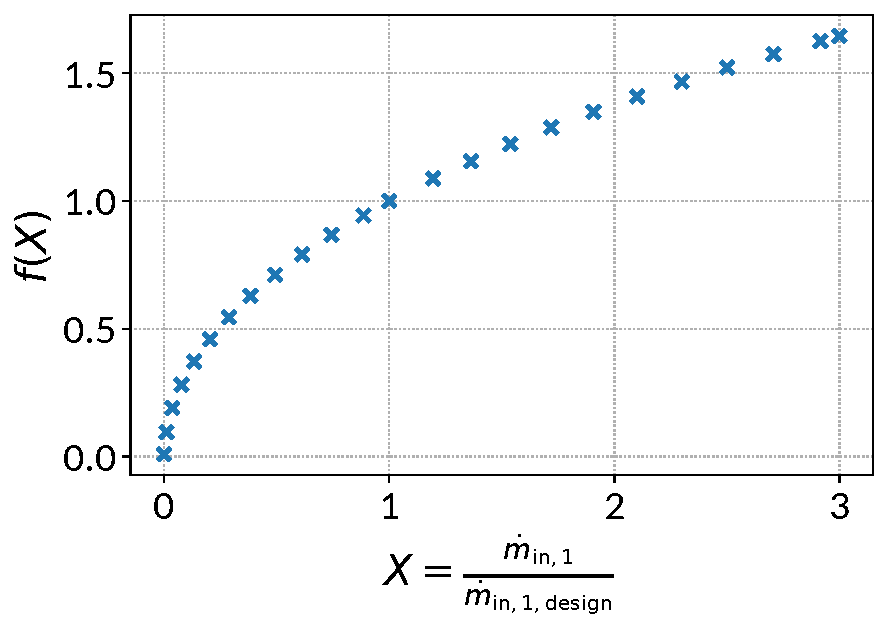
\includegraphics[width=\textwidth]{figures/HeatExchanger_CharLine_kA_char1_superheater.pdf}
\caption{Characteristics of superheater (eq. \ref{eq:HeatExchanger_kA_char})}
\label{fig:CharLine_kA_char1_superheater}
\end{center}\end{figure}

\end{minipage}
\begin{minipage}{0.5\textwidth}
\begin{figure}[H]\begin{center}
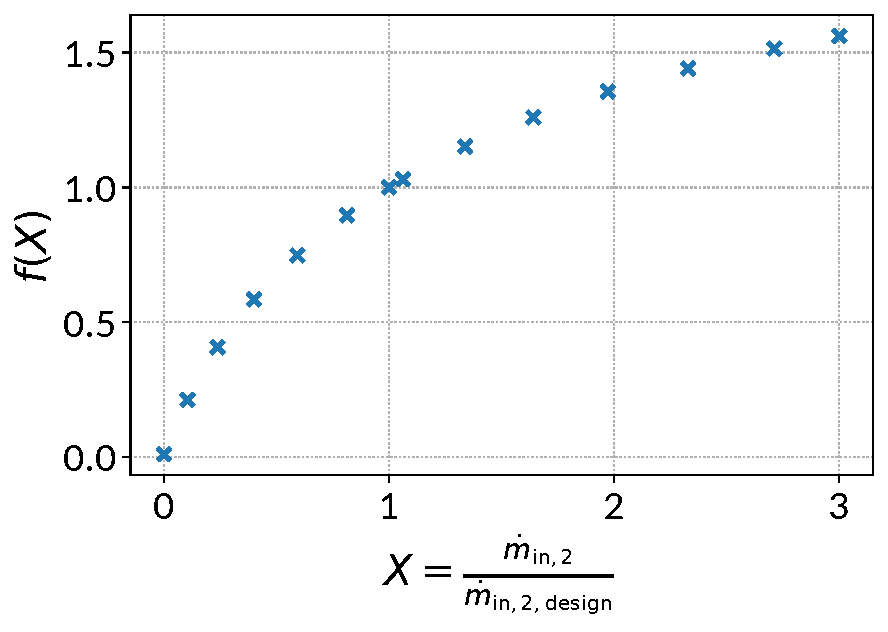
\includegraphics[width=\textwidth]{figures/HeatExchanger_CharLine_kA_char2_superheater.pdf}
\caption{Characteristics of superheater (eq. \ref{eq:HeatExchanger_kA_char})}
\label{fig:CharLine_kA_char2_superheater}
\end{center}\end{figure}

\end{minipage}

\begin{minipage}{0.5\textwidth}
\begin{figure}[H]\begin{center}
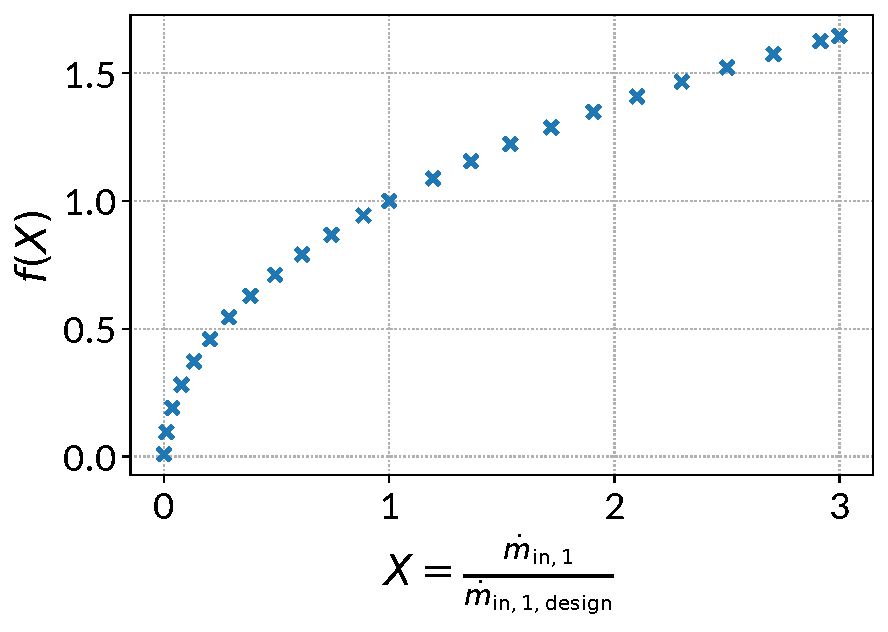
\includegraphics[width=\textwidth]{figures/HeatExchanger_CharLine_kA_char1_evaporator.pdf}
\caption{Characteristics of evaporator (eq. \ref{eq:HeatExchanger_kA_char})}
\label{fig:CharLine_kA_char1_evaporator}
\end{center}\end{figure}

\end{minipage}
\begin{minipage}{0.5\textwidth}
\begin{figure}[H]\begin{center}
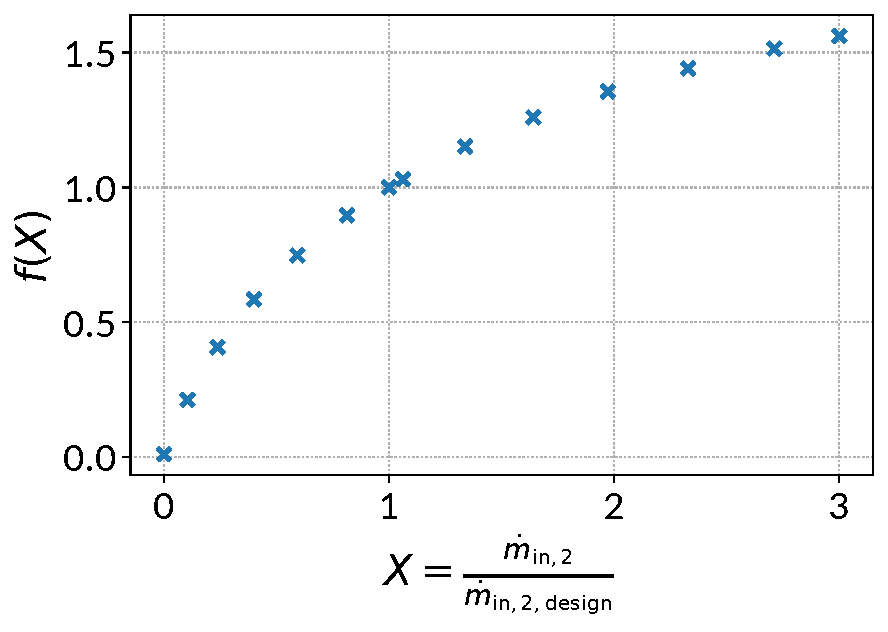
\includegraphics[width=\textwidth]{figures/HeatExchanger_CharLine_kA_char2_evaporator.pdf}
\caption{Characteristics of evaporator (eq. \ref{eq:HeatExchanger_kA_char})}
\label{fig:CharLine_kA_char2_evaporator}
\end{center}\end{figure}

\end{minipage}

\begin{minipage}{0.5\textwidth}
\begin{figure}[H]\begin{center}
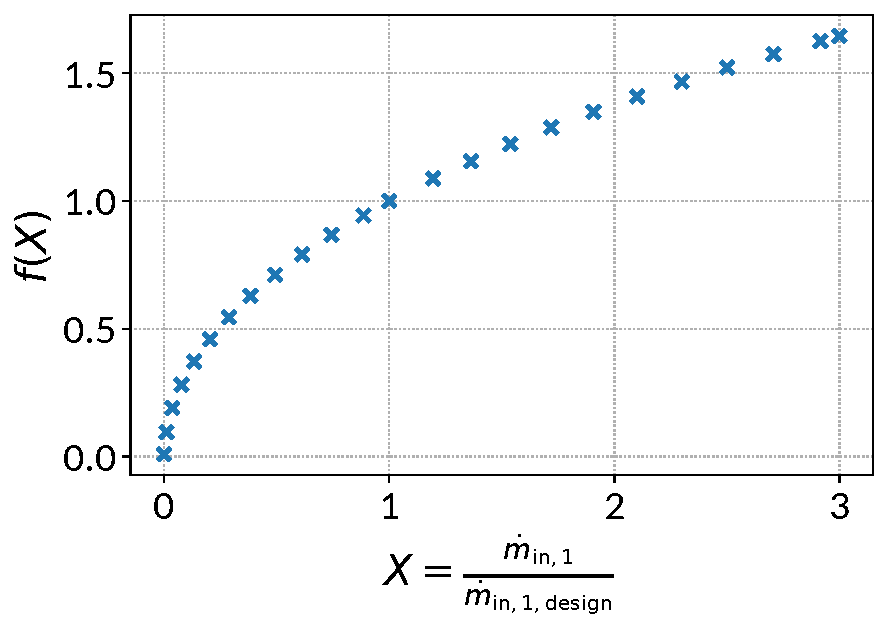
\includegraphics[width=\textwidth]{figures/HeatExchanger_CharLine_kA_char1_economizer.pdf}
\caption{Characteristics of economizer (eq. \ref{eq:HeatExchanger_kA_char})}
\label{fig:CharLine_kA_char1_economizer}
\end{center}\end{figure}

\end{minipage}
\begin{minipage}{0.5\textwidth}
\begin{figure}[H]\begin{center}
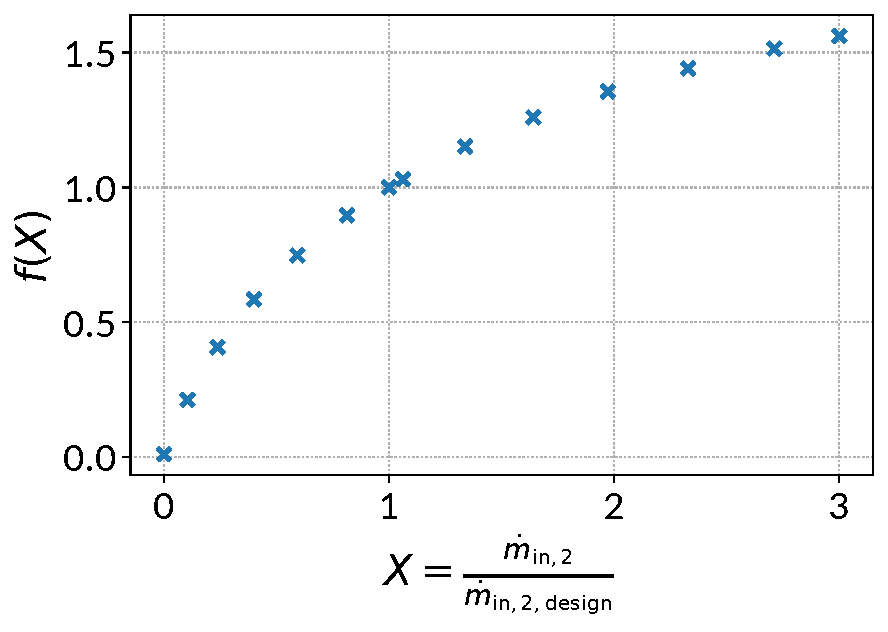
\includegraphics[width=\textwidth]{figures/HeatExchanger_CharLine_kA_char2_economizer.pdf}
\caption{Characteristics of economizer (eq. \ref{eq:HeatExchanger_kA_char})}
\label{fig:CharLine_kA_char2_economizer}
\end{center}\end{figure}

\end{minipage}


\subsection{Components of type Drum}

\subsubsection{Mandatory constraints}

\begin{equation}
\label{eq:Drum_mass_flow_constraints}
0 =\sum\dot{m}_{\mathrm{in},i}-\sum\dot{m}_{\mathrm{out},j}\;\forall i \in \text{inlets}, \forall j \in \text{outlets}
\end{equation}

\begin{equation}
\label{eq:Drum_fluid_constraints}
0 = x_{fl\mathrm{,in,1}} - x_{fl\mathrm{,out,}j}\; \forall fl \in \text{network fluids,} \; \forall j \in\text{outlets}
\end{equation}

\begin{equation}
\label{eq:Drum_energy_balance_constraints}
0=\sum_i\left(\dot{m}_{\mathrm{in,}i}\cdot h_{\mathrm{in,}i}\right) - \sum_j \left(\dot{m}_{\mathrm{out,}j} \cdot h_{\mathrm{out,}j} \right) \; \forall i \in \text{inlets} \;\forall j \in \text{outlets}
\end{equation}

\begin{equation}
\label{eq:Drum_pressure_constraints}
\begin{split}
0 = p_\mathrm{in,1} - p_{\mathrm{in,}i} & \; \forall i \in \text{inlets} \setminus \left\lbrace 1\right\rbrace\\
0 = p_\mathrm{in,1} - p_{\mathrm{out,}j} & \; \forall j \in \text{outlets}\\
\end{split}
\end{equation}

\begin{equation}
\label{eq:Drum_outlet_constraints}
\begin{split}
0 =&h_\mathrm{out,1} -h\left(p_\mathrm{out,1}, x=0\right)\\0 =&h_\mathrm{out,2} -h\left(p_\mathrm{out,2}, x=1\right)\\\end{split}
\end{equation}


\subsection{Components of type Splitter}

\subsubsection{Mandatory constraints}

\begin{equation}
\label{eq:Splitter_mass_flow_constraints}
0 =\sum\dot{m}_{\mathrm{in},i}-\sum\dot{m}_{\mathrm{out},j}\;\forall i \in \text{inlets}, \forall j \in \text{outlets}
\end{equation}

\begin{equation}
\label{eq:Splitter_fluid_constraints}
0 = x_{fl\mathrm{,in}} - x_{fl\mathrm{,out,}j}\; \forall fl \in \text{network fluids,} \; \forall j \in\text{outlets}
\end{equation}

\begin{equation}
\label{eq:Splitter_energy_balance_constraints}
0=h_{in}-h_{\mathrm{out,}j}\;\forall j \in\text{outlets}
\end{equation}

\begin{equation}
\label{eq:Splitter_pressure_constraints}
\begin{split}
0 = p_\mathrm{in,1} - p_{\mathrm{in,}i} & \; \forall i \in \text{inlets} \setminus \left\lbrace 1\right\rbrace\\
0 = p_\mathrm{in,1} - p_{\mathrm{out,}j} & \; \forall j \in \text{outlets}\\
\end{split}
\end{equation}


\subsection{Components of type Condenser}

\subsubsection{Mandatory constraints}

\begin{equation}
\label{eq:Condenser_mass_flow_constraints}
0=\dot{m}_{\mathrm{in,}i}-\dot{m}_{\mathrm{out,}i}\; \forall i \in [1, 2]
\end{equation}

\begin{equation}
\label{eq:Condenser_fluid_constraints}
0=x_{fl\mathrm{,in,}i}-x_{fl\mathrm{,out,}i}\;\forall fl \in\text{network fluids,}\; \forall i \in [1, 2]
\end{equation}

\begin{equation}
\label{eq:Condenser_energy_balance_constraints}
0 = \dot{m}_\mathrm{in,1} \cdot \left(h_\mathrm{out,1} - h_\mathrm{in,1} \right) +\dot{m}_\mathrm{in,2} \cdot \left(h_\mathrm{out,2} - h_\mathrm{in,2} \right)
\end{equation}


\subsubsection{Inputs specified}

\begin{table}[H]\begin{center}
\begin{tabular}{lrrll}
\toprule
                      label &  pr1 (\ref{eq:Condenser_pr1}) &  zeta2 (\ref{eq:Condenser_zeta2}) &  kA\_char (\ref{eq:Condenser_kA_char}) &  subcooling (\ref{eq:Condenser_subcooling}) \\
\midrule
 district heating condenser &                         0.990 &                           120.302 &                                   True &                                        True \\
                  condenser &                         0.990 &                             8.358 &                                   True &                                        True \\
\bottomrule
\end{tabular}
\caption{Parameters of components of type Condenser}
\end{center}\end{table}

\subsubsection{Equations applied}

\begin{equation}
\label{eq:Condenser_pr1}
0=p_\mathrm{in,1}\cdot pr1 - p_\mathrm{out,1}
\end{equation}

\begin{equation}
\label{eq:Condenser_zeta2}
0 = \begin{cases}
p_\mathrm{in,2}- p_\mathrm{out,2} & |\dot{m}_\mathrm{in,2}| < \unitfrac[0.0001]{kg}{s} \\
\frac{\zeta}{D^4}-\frac{(p_\mathrm{in,2}-p_\mathrm{out,2})\cdot\pi^2}{8\cdot\dot{m}_\mathrm{in,2}\cdot|\dot{m}_\mathrm{in,2}|\cdot\frac{v_\mathrm{in,2} + v_\mathrm{out,2}}{2}}& |\dot{m}_\mathrm{in,2}| \geq \unitfrac[0.0001]{kg}{s}
\end{cases}
\end{equation}

\begin{equation}
\label{eq:Condenser_kA_char}
\begin{split}
0 = & \dot{m}_\mathrm{in,1} \cdot \left( h_\mathrm{out,1} - h_\mathrm{in,1}\right)\\
&+kA_\mathrm{design} \cdot f_\mathrm{kA} \cdot \frac{T_\mathrm{out,1} - T_\mathrm{in,2} - T_\mathrm{sat}\left( p_\mathrm{in,1}\right) +T_\mathrm{out,2}}{\ln{\frac{T_\mathrm{out,1}-T_\mathrm{in,2}}{T_\mathrm{sat}\left( p_\mathrm{in,1}\right)- T_\mathrm{out,2}}}}\\
f_\mathrm{kA}=&\frac{2}{\frac{1}{f\left(X_2\right)}+\frac{1}{f\left(X_2\right)}}\\
\end{split}
\end{equation}

\begin{equation}
\label{eq:Condenser_subcooling}
0=h_\mathrm{out,1} -h\left(p_\mathrm{out,1}, x=0 \right)
\end{equation}

\begin{minipage}{0.5\textwidth}
\begin{figure}[H]\begin{center}
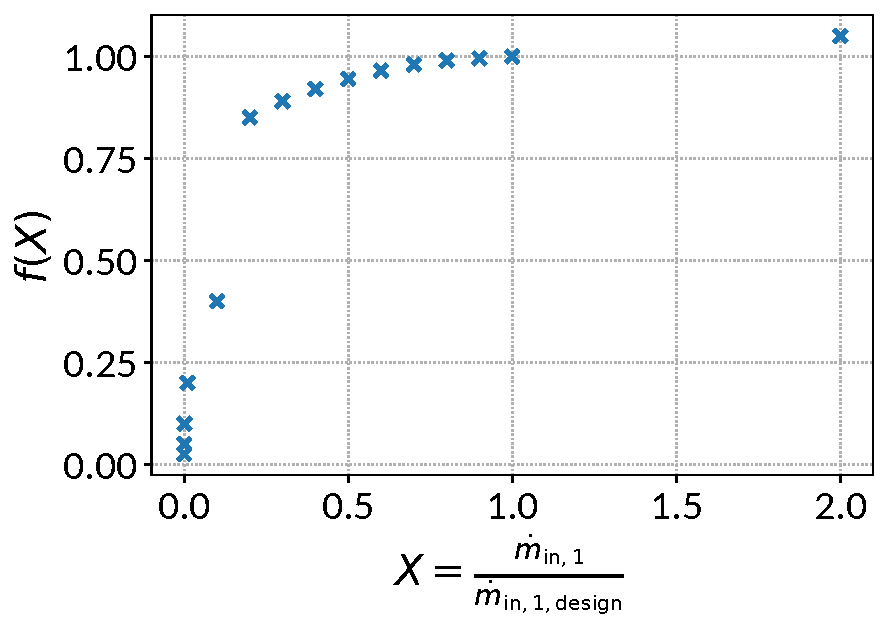
\includegraphics[width=\textwidth]{figures/Condenser_CharLine_kA_char1_district_heating_condenser.pdf}
\caption{Characteristics of district heating condenser (eq. \ref{eq:Condenser_kA_char})}
\label{fig:CharLine_kA_char1_district heating condenser}
\end{center}\end{figure}

\end{minipage}
\begin{minipage}{0.5\textwidth}
\begin{figure}[H]\begin{center}
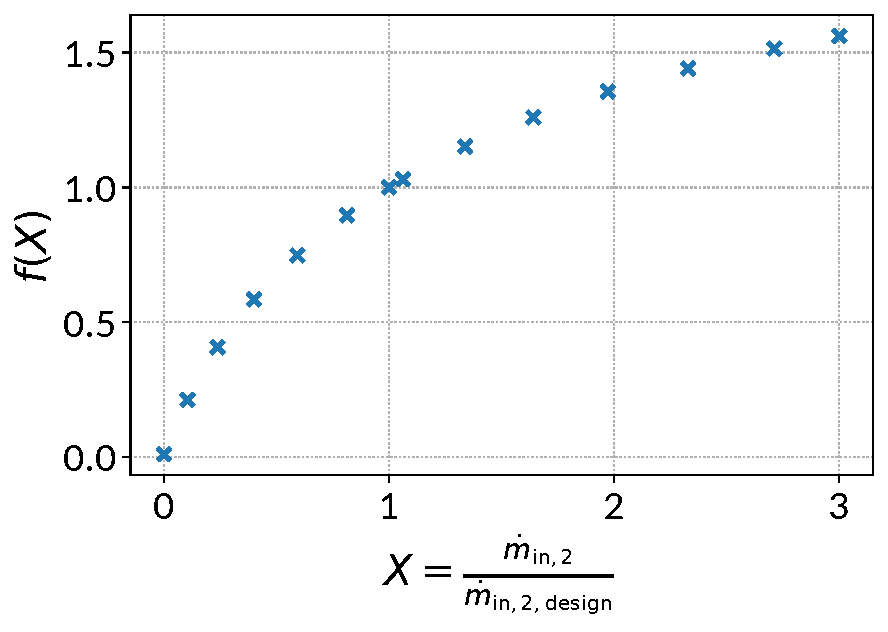
\includegraphics[width=\textwidth]{figures/Condenser_CharLine_kA_char2_district_heating_condenser.pdf}
\caption{Characteristics of district heating condenser (eq. \ref{eq:Condenser_kA_char})}
\label{fig:CharLine_kA_char2_district heating condenser}
\end{center}\end{figure}

\end{minipage}

\begin{minipage}{0.5\textwidth}
\begin{figure}[H]\begin{center}
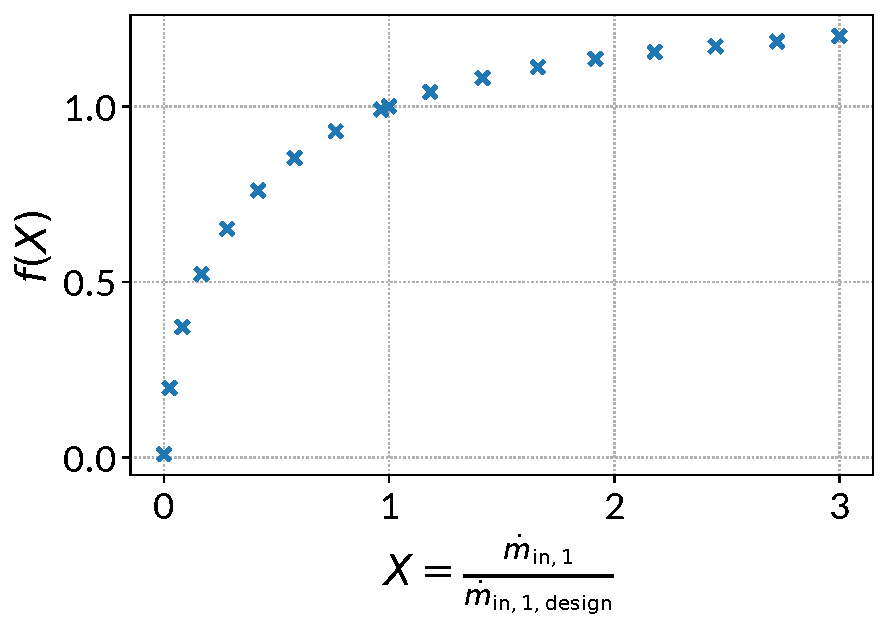
\includegraphics[width=\textwidth]{figures/Condenser_CharLine_kA_char1_condenser.pdf}
\caption{Characteristics of condenser (eq. \ref{eq:Condenser_kA_char})}
\label{fig:CharLine_kA_char1_condenser}
\end{center}\end{figure}

\end{minipage}
\begin{minipage}{0.5\textwidth}
\begin{figure}[H]\begin{center}
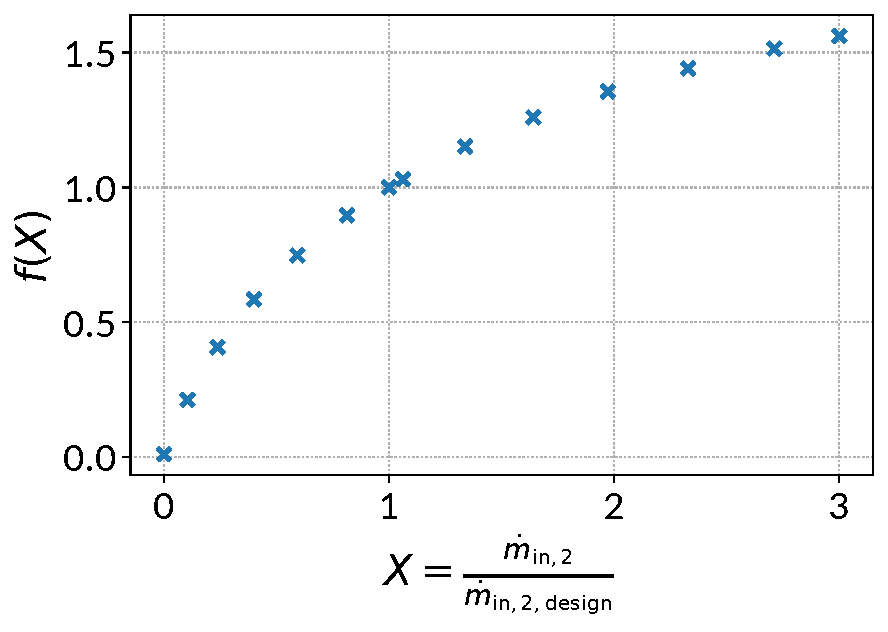
\includegraphics[width=\textwidth]{figures/Condenser_CharLine_kA_char2_condenser.pdf}
\caption{Characteristics of condenser (eq. \ref{eq:Condenser_kA_char})}
\label{fig:CharLine_kA_char2_condenser}
\end{center}\end{figure}

\end{minipage}


\subsection{Components of type Pump}

\subsubsection{Mandatory constraints}

\begin{equation}
\label{eq:Pump_mass_flow_constraints}
0=\dot{m}_{\mathrm{in,}i}-\dot{m}_{\mathrm{out,}i}\; \forall i \in [1]
\end{equation}

\begin{equation}
\label{eq:Pump_fluid_constraints}
0=x_{fl\mathrm{,in,}i}-x_{fl\mathrm{,out,}i}\;\forall fl \in\text{network fluids,}\; \forall i \in [1]
\end{equation}


\subsubsection{Inputs specified}

\begin{table}[H]\begin{center}
\begin{tabular}{ll}
\toprule
             label &  eta\_s\_char (\ref{eq:Pump_eta_s_char}) \\
\midrule
 feed water pump 1 &                                     True \\
 feed water pump 2 &                                     True \\
\bottomrule
\end{tabular}
\caption{Parameters of components of type Pump}
\end{center}\end{table}

\subsubsection{Equations applied}

\begin{equation}
\label{eq:Pump_eta_s_char}
0=\left(h_\mathrm{out}-h_\mathrm{in}\right)\cdot\eta_\mathrm{s,design}\cdot f\left( X \right)-\left( h_{out,s} - h_{in} \right)
\end{equation}

\begin{minipage}{0.5\textwidth}
\begin{figure}[H]\begin{center}
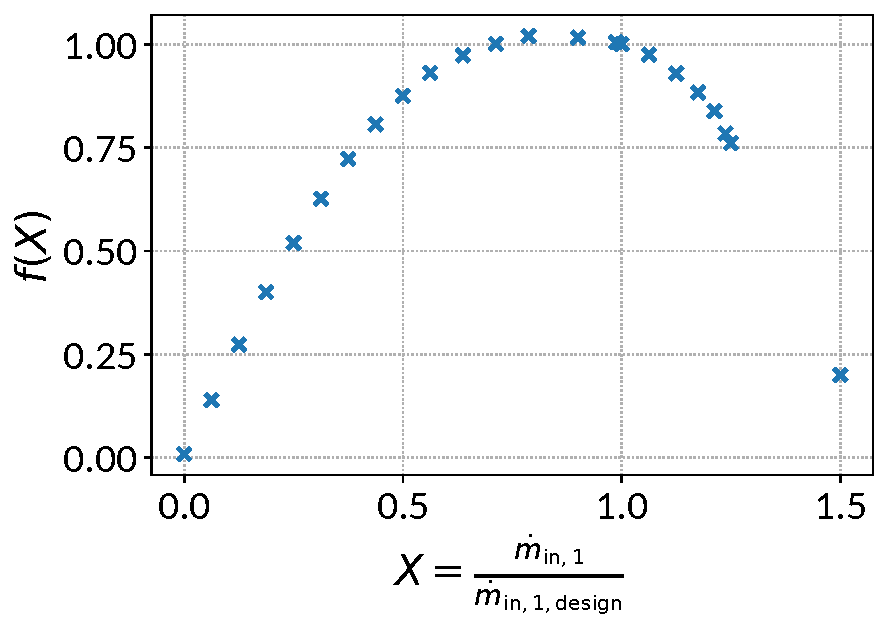
\includegraphics[width=\textwidth]{figures/Pump_CharLine_eta_s_char_feed_water_pump_1.pdf}
\caption{Characteristics of feed water pump 1 (eq. \ref{eq:Pump_eta_s_char})}
\label{fig:CharLine_eta_s_char_feed water pump 1}
\end{center}\end{figure}

\end{minipage}
\begin{minipage}{0.5\textwidth}
\begin{figure}[H]\begin{center}
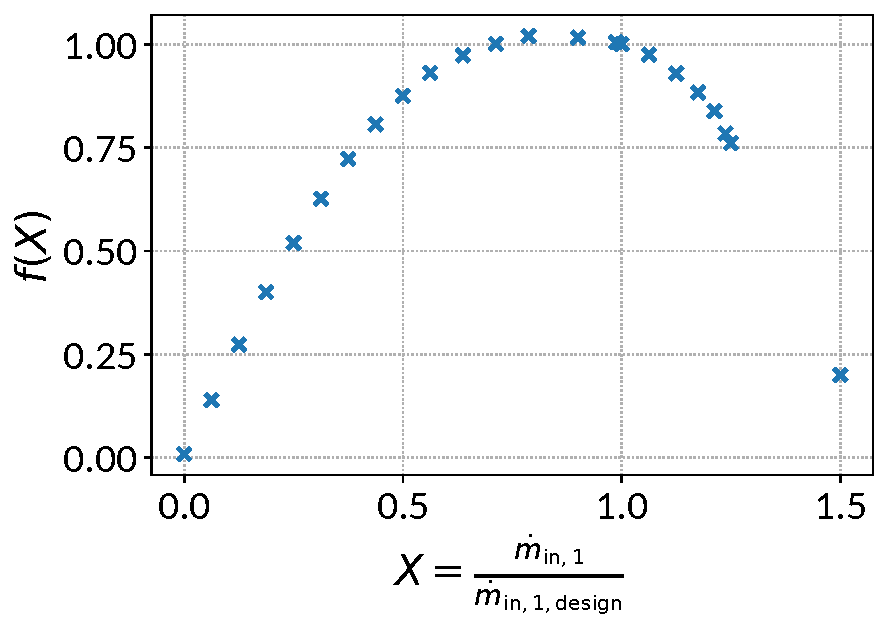
\includegraphics[width=\textwidth]{figures/Pump_CharLine_eta_s_char_feed_water_pump_2.pdf}
\caption{Characteristics of feed water pump 2 (eq. \ref{eq:Pump_eta_s_char})}
\label{fig:CharLine_eta_s_char_feed water pump 2}
\end{center}\end{figure}

\end{minipage}


\subsection{Components of type Merge}

\subsubsection{Mandatory constraints}

\begin{equation}
\label{eq:Merge_mass_flow_constraints}
0 =\sum\dot{m}_{\mathrm{in},i}-\sum\dot{m}_{\mathrm{out},j}\;\forall i \in \text{inlets}, \forall j \in \text{outlets}
\end{equation}

\begin{equation}
\label{eq:Merge_fluid_constraints}
0=\sum_i \dot{m}_{\mathrm{in,}i} \cdot x_{fl\mathrm{,in,}i}- \dot {m}_\mathrm{out} \cdot x_{fl\mathrm{,out}}\; \forall fl \in \text{network fluids,} \; \forall i \in\text{inlets}
\end{equation}

\begin{equation}
\label{eq:Merge_energy_balance_constraints}
0=\sum_i\left(\dot{m}_{\mathrm{in,}i}\cdot h_{\mathrm{in,}i}\right) - \dot{m}_\mathrm{out} \cdot h_\mathrm{out} \; \forall i \in \text{inlets}
\end{equation}

\begin{equation}
\label{eq:Merge_pressure_constraints}
\begin{split}
0 = p_\mathrm{in,1} - p_{\mathrm{in,}i} & \; \forall i \in \text{inlets} \setminus \left\lbrace 1\right\rbrace\\
0 = p_\mathrm{in,1} - p_{\mathrm{out,}j} & \; \forall j \in \text{outlets}\\
\end{split}
\end{equation}


\subsection{Components of type Valve}

\subsubsection{Mandatory constraints}

\begin{equation}
\label{eq:Valve_mass_flow_constraints}
0=\dot{m}_{\mathrm{in,}i}-\dot{m}_{\mathrm{out,}i}\; \forall i \in [1]
\end{equation}

\begin{equation}
\label{eq:Valve_fluid_constraints}
0=x_{fl\mathrm{,in,}i}-x_{fl\mathrm{,out,}i}\;\forall fl \in\text{network fluids,}\; \forall i \in [1]
\end{equation}

\begin{equation}
\label{eq:Valve_enthalpy_equality_constraints}
0=h_{\mathrm{in,}i}-h_{\mathrm{out,}i}\; \forall i \in [1]
\end{equation}


\section{Busses in offdesign mode}

\subsection{Bus ``power output''}

This bus is used for postprocessing only.

\begin{table}[H]\begin{center}
\begin{tabular}{llll}
\toprule
                       label &                                                   $\dot{E}_\mathrm{comp}$ &                $\dot{E}_\mathrm{bus}$ &                                                               $\eta$ \\
\midrule
                 gas turbine &  $\dot{m}_\mathrm{in} \cdot \left(h_\mathrm{out} - h_\mathrm{in} \right)$ &    $\dot{E}_\mathrm{comp} \cdot \eta$ &      $f\left(X\right)$ (\ref{fig:Bus_CharLine_gas turbineoffdesign}) \\
                  compressor &  $\dot{m}_\mathrm{in} \cdot \left(h_\mathrm{out} - h_\mathrm{in} \right)$ &    $\dot{E}_\mathrm{comp} \cdot \eta$ &                                                                1.000 \\
             fuel compressor &  $\dot{m}_\mathrm{in} \cdot \left(h_\mathrm{out} - h_\mathrm{in} \right)$ &  $\frac{\dot{E}_\mathrm{comp}}{\eta}$ &  $f\left(X\right)$ (\ref{fig:Bus_CharLine_fuel compressoroffdesign}) \\
 steam turbine high pressure &  $\dot{m}_\mathrm{in} \cdot \left(h_\mathrm{out} - h_\mathrm{in} \right)$ &    $\dot{E}_\mathrm{comp} \cdot \eta$ &      $f\left(X\right)$ (\ref{fig:Bus_CharLine_gas turbineoffdesign}) \\
           feed water pump 1 &  $\dot{m}_\mathrm{in} \cdot \left(h_\mathrm{out} - h_\mathrm{in} \right)$ &  $\frac{\dot{E}_\mathrm{comp}}{\eta}$ &  $f\left(X\right)$ (\ref{fig:Bus_CharLine_fuel compressoroffdesign}) \\
  steam turbine low pressure &  $\dot{m}_\mathrm{in} \cdot \left(h_\mathrm{out} - h_\mathrm{in} \right)$ &    $\dot{E}_\mathrm{comp} \cdot \eta$ &      $f\left(X\right)$ (\ref{fig:Bus_CharLine_gas turbineoffdesign}) \\
           feed water pump 2 &  $\dot{m}_\mathrm{in} \cdot \left(h_\mathrm{out} - h_\mathrm{in} \right)$ &  $\frac{\dot{E}_\mathrm{comp}}{\eta}$ &  $f\left(X\right)$ (\ref{fig:Bus_CharLine_fuel compressoroffdesign}) \\
\bottomrule
\end{tabular}
\caption{power output}
\end{center}\end{table}



\begin{minipage}{0.5\textwidth}
\begin{figure}[H]\begin{center}
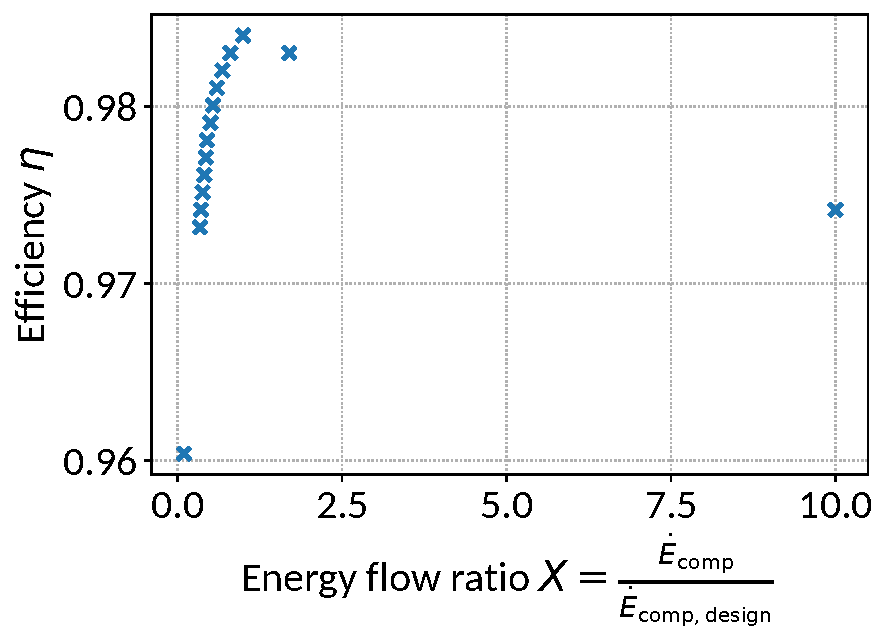
\includegraphics[width=\textwidth]{figures/Bus_CharLine_gas_turbineoffdesign.pdf}
\caption{Bus efficiency characteristic}
\label{fig:Bus_CharLine_gas turbineoffdesign}
\end{center}\end{figure}

\end{minipage}
\begin{minipage}{0.5\textwidth}
\begin{figure}[H]\begin{center}
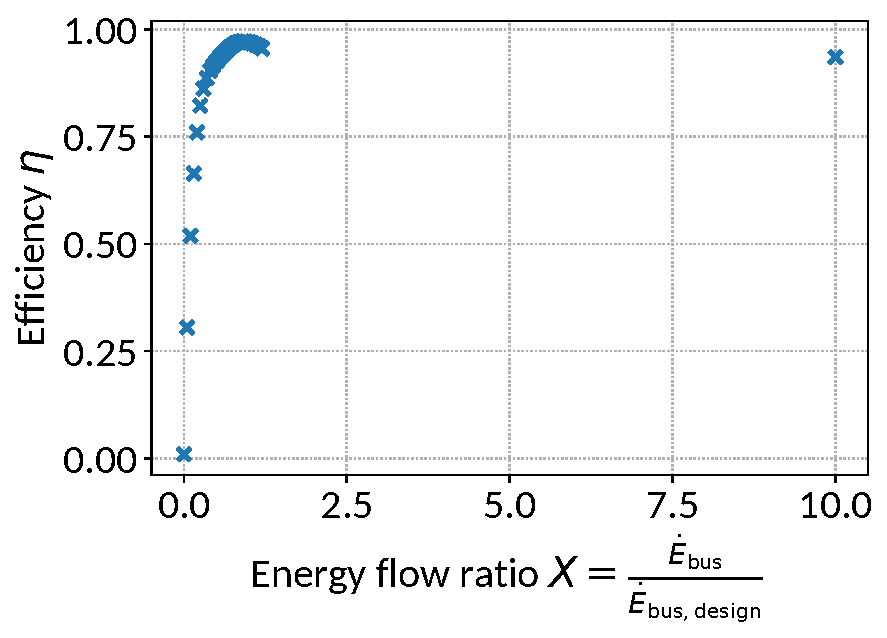
\includegraphics[width=\textwidth]{figures/Bus_CharLine_fuel_compressoroffdesign.pdf}
\caption{Bus efficiency characteristic}
\label{fig:Bus_CharLine_fuel compressoroffdesign}
\end{center}\end{figure}

\end{minipage}


\subsection{Bus ``gas turbine power output''}

Specified total value of energy flow: $\dot{E}_\mathrm{bus} = \unit[-105822240.972]{W}$

\begin{equation}
\label{eq:Bus_energy_flow_sum}
0=\dot{E}_\mathrm{bus} -\sum_i \dot{E}_{\mathrm{bus,}i}
\end{equation}

\begin{table}[H]\begin{center}
\begin{tabular}{llll}
\toprule
       label &                                                   $\dot{E}_\mathrm{comp}$ &              $\dot{E}_\mathrm{bus}$ & $\eta$ \\
\midrule
 gas turbine &  $\dot{m}_\mathrm{in} \cdot \left(h_\mathrm{out} - h_\mathrm{in} \right)$ &  $\dot{E}_\mathrm{comp} \cdot \eta$ &  1.000 \\
  compressor &  $\dot{m}_\mathrm{in} \cdot \left(h_\mathrm{out} - h_\mathrm{in} \right)$ &  $\dot{E}_\mathrm{comp} \cdot \eta$ &  1.000 \\
\bottomrule
\end{tabular}
\caption{gas turbine power output}
\end{center}\end{table}




\subsection{Bus ``heat output''}

Specified total value of energy flow: $\dot{E}_\mathrm{bus} = \unit[-10000000.000]{W}$

\begin{equation}
\label{eq:Bus_energy_flow_sum}
0=\dot{E}_\mathrm{bus} -\sum_i \dot{E}_{\mathrm{bus,}i}
\end{equation}

\begin{table}[H]\begin{center}
\begin{tabular}{llll}
\toprule
                      label &                                                         $\dot{E}_\mathrm{comp}$ &              $\dot{E}_\mathrm{bus}$ & $\eta$ \\
\midrule
 district heating condenser &  $\dot{m}_\mathrm{in,1} \cdot \left(h_\mathrm{out,1} - h_\mathrm{in,1} \right)$ &  $\dot{E}_\mathrm{comp} \cdot \eta$ &  1.000 \\
\bottomrule
\end{tabular}
\caption{heat output}
\end{center}\end{table}




\subsection{Bus ``heat cond''}

This bus is used for postprocessing only.

\begin{table}[H]\begin{center}
\begin{tabular}{llll}
\toprule
     label &                                                         $\dot{E}_\mathrm{comp}$ &              $\dot{E}_\mathrm{bus}$ & $\eta$ \\
\midrule
 condenser &  $\dot{m}_\mathrm{in,1} \cdot \left(h_\mathrm{out,1} - h_\mathrm{in,1} \right)$ &  $\dot{E}_\mathrm{comp} \cdot \eta$ &  1.000 \\
\bottomrule
\end{tabular}
\caption{heat cond}
\end{center}\end{table}




\subsection{Bus ``heat input''}

This bus is used for postprocessing only.

\begin{table}[H]\begin{center}
\begin{tabular}{llll}
\toprule
      label &                                                                                                                                               $\dot{E}_\mathrm{comp}$ &              $\dot{E}_\mathrm{bus}$ & $\eta$ \\
\midrule
 combustion &  $LHV_\mathrm{fuel} \cdot \left[\sum_i \left(\dot{m}_{\mathrm{in,}i}\cdot x_{\mathrm{fuel,in,}i}\right)- \dot{m}_\mathrm{out,1}\cdot x_{\mathrm{fuel,out,}1} \right]$ &  $\dot{E}_\mathrm{comp} \cdot \eta$ &  1.000 \\
\bottomrule
\end{tabular}
\caption{heat input}
\end{center}\end{table}




